%package list
\documentclass{article}
\usepackage[top=3cm, bottom=3cm, outer=3cm, inner=3cm]{geometry}
\usepackage{multicol}
\usepackage{graphicx}
\usepackage{url}
%\usepackage{cite}
\usepackage{hyperref}
\usepackage{array}
%\usepackage{multicol}
\newcolumntype{x}[1]{>{\centering\arraybackslash\hspace{0pt}}p{#1}}
\usepackage{natbib}
\usepackage{pdfpages}
\usepackage{multirow}
\usepackage[normalem]{ulem}
\useunder{\uline}{\ul}{}
\usepackage{svg}
\usepackage{xcolor}
\usepackage{listings}
\lstdefinestyle{ascii-tree}{
    literate={├}{|}1 {─}{--}1 {└}{+}1 
  }
\lstset{basicstyle=\ttfamily,
  showstringspaces=false,
  commentstyle=\color{red},
  keywordstyle=\color{blue}
}
%\usepackage{booktabs}
\usepackage[labelformat=empty]{caption}
\usepackage{subcaption}
\usepackage{float}
\usepackage{array}

\newcolumntype{M}[1]{>{\centering\arraybackslash}m{#1}}
\newcolumntype{N}{@{}m{0pt}@{}}


%%%%%%%%%%%%%%%%%%%%%%%%%%%%%%%%%%%%%%%%%%%%%%%%%%%%%%%%%%%%%%%%%%%%%%%%%%%%
%%%%%%%%%%%%%%%%%%%%%%%%%%%%%%%%%%%%%%%%%%%%%%%%%%%%%%%%%%%%%%%%%%%%%%%%%%%%
\newcommand{\itemEmail}{cmestasz@unsa.edu.pe}
\newcommand{\itemStudent}{Christian Mestas Zegarra}
\newcommand{\itemCourse}{Fundamentos de la Programación 2}
\newcommand{\itemCourseCode}{1701213}
\newcommand{\itemSemester}{II}
\newcommand{\itemUniversity}{Universidad Nacional de San Agustín de Arequipa}
\newcommand{\itemFaculty}{Facultad de Ingeniería de Producción y Servicios}
\newcommand{\itemDepartment}{Departamento Académico de Ingeniería de Sistemas e Informática}
\newcommand{\itemSchool}{Escuela Profesional de Ingeniería de Sistemas}
\newcommand{\itemAcademic}{2023 - B}
\newcommand{\itemInput}{Del 13 Setiembre 2023}
\newcommand{\itemOutput}{Al 20 Setiembre 2023}
\newcommand{\itemPracticeNumber}{01}
\newcommand{\itemTheme}{Arreglos estándar}
%%%%%%%%%%%%%%%%%%%%%%%%%%%%%%%%%%%%%%%%%%%%%%%%%%%%%%%%%%%%%%%%%%%%%%%%%%%%
%%%%%%%%%%%%%%%%%%%%%%%%%%%%%%%%%%%%%%%%%%%%%%%%%%%%%%%%%%%%%%%%%%%%%%%%%%%%

\usepackage[english,spanish]{babel}
\usepackage[utf8]{inputenc}
\AtBeginDocument{\selectlanguage{spanish}}
\renewcommand{\figurename}{Figura}
\renewcommand{\refname}{Referencias}
\renewcommand{\tablename}{Tabla} %esto no funciona cuando se usa babel
\AtBeginDocument{%
	\renewcommand\tablename{Tabla}
}

\usepackage{fancyhdr}
\pagestyle{fancy}
\fancyhf{}
\setlength{\headheight}{30pt}
\renewcommand{\headrulewidth}{1pt}
\renewcommand{\footrulewidth}{1pt}
\fancyhead[L]{\raisebox{-0.2\height}{
\includegraphics[width=3cm]{img/logo_episunsa.png}}}
\fancyhead[C]{\fontsize{7}{7}\selectfont	\itemUniversity \\ \itemFaculty \\ \itemDepartment \\ \itemSchool \\ \textbf{\itemCourse}}
\fancyhead[R]{\raisebox{-0.2\height}{
\includegraphics[width=1.2cm]{img/logo_abet}}}
\fancyfoot[L]{Christian Mestas}
\fancyfoot[C]{\itemCourse}
\fancyfoot[R]{Página \thepage}

% para el codigo fuente
\usepackage{listings}
\usepackage{color, colortbl}
\definecolor{dkgreen}{rgb}{0,0.6,0}
\definecolor{gray}{rgb}{0.5,0.5,0.5}
\definecolor{mauve}{rgb}{0.58,0,0.82}
\definecolor{codebackground}{rgb}{0.95, 0.95, 0.92}
\definecolor{tablebackground}{rgb}{0.8, 0, 0}

\lstset{frame=tb,
	language=bash,
	aboveskip=3mm,
	belowskip=3mm,
	showstringspaces=false,
	columns=flexible,
	basicstyle={\small\ttfamily},
	numbers=none,
	numberstyle=\tiny\color{gray},
	keywordstyle=\color{blue},
	commentstyle=\color{dkgreen},
	stringstyle=\color{mauve},
	breaklines=true,
	breakatwhitespace=true,
	tabsize=3,
	backgroundcolor= \color{codebackground},
}

\begin{document}

\vspace*{10px}

\begin{center}
	\fontsize{17}{17} \textbf{ Informe de Laboratorio \itemPracticeNumber}
\end{center}
\centerline{\textbf{\Large Tema: \itemTheme}}
%\vspace*{0.5cm}	

\begin{flushright}
	\begin{tabular}{|M{2.5cm}|N|}
		\hline
		\rowcolor{tablebackground}
		\color{white} \textbf{Nota} \\
		\hline
		\\[30pt]
		\hline
	\end{tabular}
\end{flushright}

\begin{table}[H]
	\begin{tabular}{|M{4.7cm}|M{4.8cm}|M{4.8cm}|}
		\hline
		\rowcolor{tablebackground}
		\color{white} \textbf{Estudiante} & \color{white}\textbf{Escuela} & \color{white}\textbf{Asignatura}                                        \\
		\hline
		{\itemStudent \par \itemEmail}    & \itemSchool                   & {\itemCourse \par Semestre: \itemSemester \par Código: \itemCourseCode} \\
		\hline
	\end{tabular}
\end{table}

\begin{table}[H]
	\begin{tabular}{|M{4.7cm}|M{4.8cm}|M{4.8cm}|}
		\hline
		\rowcolor{tablebackground}
		\color{white}\textbf{Laboratorio} & \color{white}\textbf{Tema} & \color{white}\textbf{Duración} \\
		\hline
		\itemPracticeNumber               & \itemTheme                 & 04 horas                       \\
		\hline
	\end{tabular}
\end{table}

\begin{table}[H]
	\begin{tabular}{|M{4.7cm}|M{4.8cm}|M{4.8cm}|}
		\hline
		\rowcolor{tablebackground}
		\color{white}\textbf{Semestre académico} & \color{white}\textbf{Fecha de inicio} & \color{white}\textbf{Fecha de entrega} \\
		\hline
		\itemAcademic                            & \itemInput                            & \itemOutput                            \\
		\hline
	\end{tabular}
\end{table}

\section{Tarea}
\begin{itemize}
	\item \textbf{Actividad 1:} Escribir un programa donde se creen 5 soldados considerando sólo su nombre. Ingresar sus datos y
	      después mostrarlos. Restricción: se realizará considerando sólo los conocimientos que se tienen de FP1 y sin utilizar arreglos estándar,
	      sólo usar variables simples.
	\item \textbf{Actividad 2:} Escribir un programa donde se creen 5 soldados considerando su nombre y nivel de vida. Ingresar sus
	      datos y después mostrarlos. Restricción: se realizará considerando sólo los conocimientos que se tienen de FP1 y sin utilizar arreglos estándar,
	      sólo usar variables simples.
	\item \textbf{Actividad 3:} Escribir un programa donde se creen 5 soldados considerando sólo su nombre. Ingresar sus datos y
	      después mostrarlos. Restricción: aplicar arreglos estándar.
	\item \textbf{Actividad 4:} Escribir un programa donde se creen 5 soldados considerando su nombre y nivel de vida. Ingresar sus
	      datos y después mostrarlos. Restricción: aplicar arreglos estándar. (Todavía no aplicar arreglo de objetos)
	\item \textbf{Actividad 5:} Escribir un programa donde se creen 2 ejércitos, cada uno con un número aleatorio de soldados entre
	      1 y 5, considerando sólo su nombre. Sus datos se inicializan automáticamente con nombres tales como “Soldado0”,
	      “Soldado1”, etc. Luego de crear los 2 ejércitos se deben mostrar los datos de todos los soldados de ambos ejércitos
	      e indicar qué ejército fue el ganador. Restricción: aplicar arreglos estándar y métodos para inicializar los ejércitos, mostrar ejército y mostrar ejército
	      ganador. La métrica a aplicar para indicar el ganador es el mayor número de soldados de cada ejército, puede
	      haber empates. (Todavía no aplicar arreglo de objetos)
\end{itemize}
\pagebreak

\section{Equipos, materiales y temas utilizados}
\begin{itemize}
	\item Sistema Operativo Microsoft Windows 10 Pro 64 bits
	\item Visual Studio Code 1.82.2
	\item Java Development Kit 17.0.1
	\item Git 2.41.0.windows.1
	\item Windows PowerShell 5.1.19041.3031
	\item Cuenta en GitHub con el correo institucional.
	\item Arreglos estándar.
\end{itemize}

\section{URL de Repositorio Github}
\begin{itemize}
	\item URL del Repositorio GitHub para clonar o recuperar.
	\item \url{https://github.com/cmestasz/fp2-23b.git}
	\item URL para el laboratorio 01 en el Repositorio GitHub.
	\item \url{https://github.com/cmestasz/fp2-23b/tree/main/fase01/lab01}
\end{itemize}

\section{Actividades con el repositorio GitHub}

\subsection{Creando e inicializando repositorio GitHub}
\begin{itemize}
	\item Como es el primer laboratorio se creo el repositorio GitHub.
	\item Se realizaron los siguientes comandos en la computadora:
\end{itemize}

\begin{lstlisting}[language=bash,caption={Creando directorio de trabajo}]
		$ mkdir cmestasz
		$ cd cmestasz
	\end{lstlisting}
\begin{lstlisting}[language=bash,caption={Creando directorio para repositorio GitHub}]
		$ mkdir fp2-23b
		$ cd fp2-23b
		$ mkdir fase01
		$ mkdir fase02
		$ mkdir fase03
		$ cd fase01
		$ mkdir lab01
		$ cd ..
	\end{lstlisting}
\begin{lstlisting}[language=bash,caption={Inicializando repositorio GitHub}]
		$ git config --global user.name "Christian Mestas Zegarra"
		$ git config --global user.email cmestasz@unsa.edu.pe
		$ git init
	\end{lstlisting}

\subsection{Commits}
\begin{lstlisting}[language=bash,caption={Creando .gitignore}]
		$ code .gitignore
	\end{lstlisting}
\begin{lstlisting}[language=bash,caption={Primer Commit / .gitignore}]
		$ git add .gitignore
		$ git commit -m "Creando .gitignore para evitar *.class"
		$ git branch -M main
		$ git remote add origin https://github.com/cmestasz/fp2-23b.git
		$ git push -u origin main
	\end{lstlisting}
Los siguientes comandos son parte de la configuración del repositorio, por lo que solo son ejecutados durante el primer commit:
\begin{itemize}
	\item \textbf{"git branch -M"} crea la rama main, en la que se trabajara posteriormente.
	\item \textbf{"git remote add origin"} configura la dirección del repositorio en línea.
	\item \textbf{"git push -u origin main"} configura la rama en la que se deben guardar los archivos.
\end{itemize}
\begin{figure}[H]
	\centering
	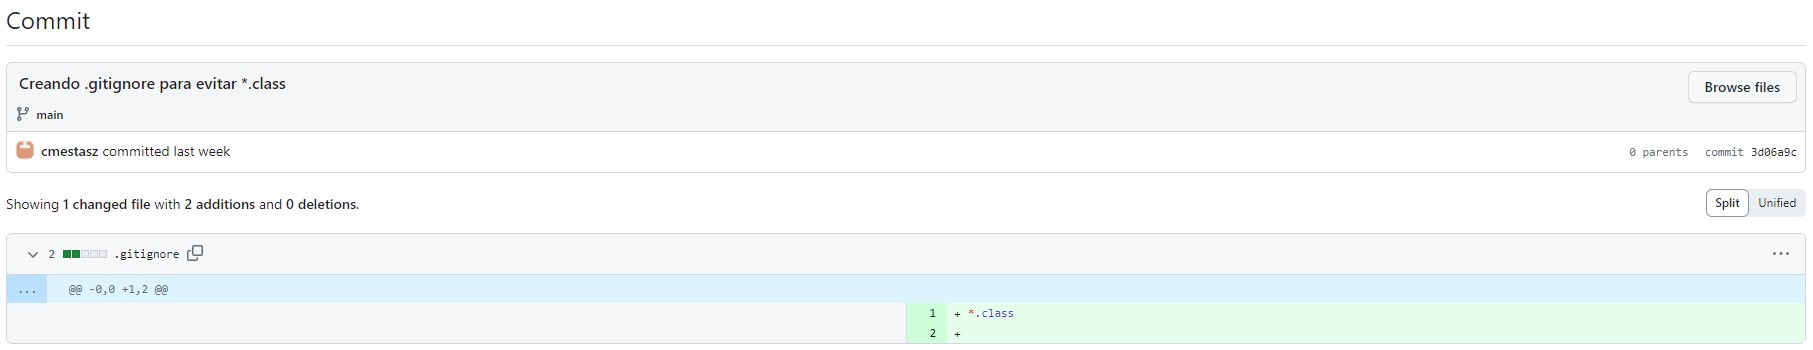
\includegraphics[width=1\textwidth,keepaspectratio]{img/commit01.jpg}
	\caption{Primer Commit.}
\end{figure}
\begin{lstlisting}[language=bash,caption={Creando VideoJuego.java}]
		$ cd fase01/lab01
		$ code VideoJuego.java
	\end{lstlisting}
\begin{lstlisting}[language=bash,caption={Segundo Commit / VideoJuego.java}]
		$ git add VideoJuego.java
		$ git commit -m "Demo de VideoJuego.java donde saluda con un mensaje"
		$ git push
	\end{lstlisting}
\begin{figure}[H]
	\centering
	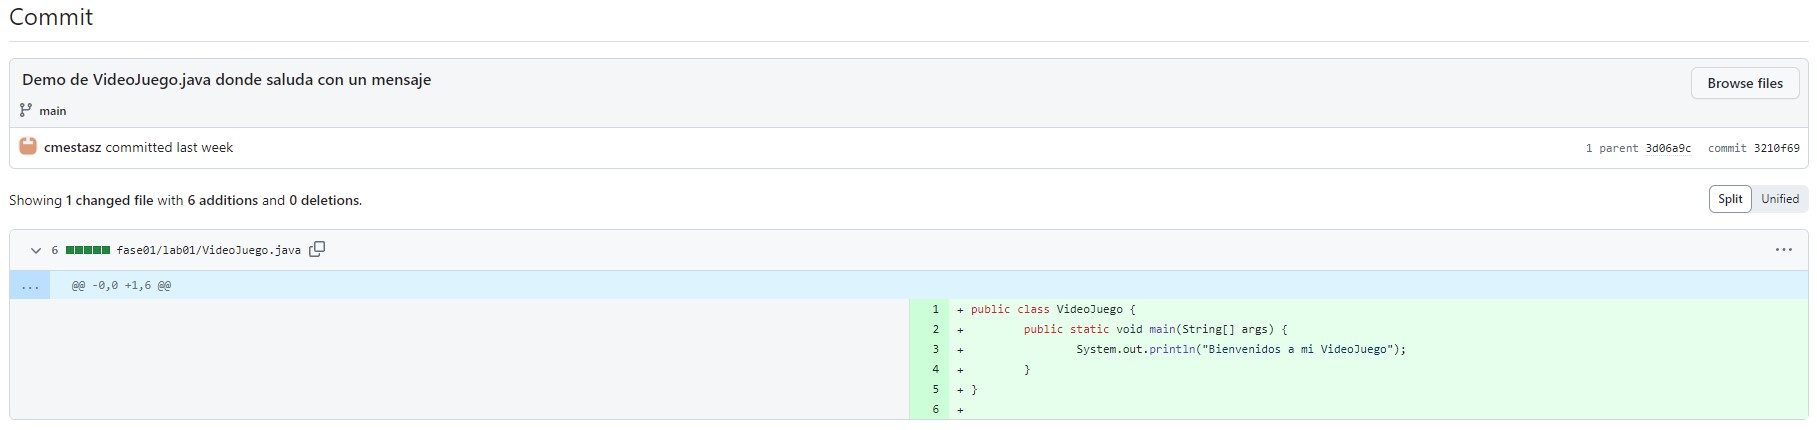
\includegraphics[width=1\textwidth,keepaspectratio]{img/commit02.jpg}
	\caption{Segundo Commit.}
\end{figure}
\begin{lstlisting}[language=bash,caption={Creando Actividades.java}]
		$ code Actividades.java
	\end{lstlisting}
\begin{lstlisting}[language=bash,caption={Tercer - Septimo Commit / Actividades.java}]
		$ git add Actividades.java
		$ git commit -m "Actividad 1"
		$ code Actividades.java
		$ git add Actividades.java
		$ git commit -m "Actividad 2"
		$ code Actividades.java
		$ git add Actividades.java
		$ git commit -m "Actividad 3"
		$ code Actividades.java
		$ git add Actividades.java
		$ git commit -m "Actividad 4"
		$ code Actividades.java
		$ git add Actividades.java
		$ git commit -m "Actividad 5"
		$ git push
	\end{lstlisting}
\begin{figure}[H]
	\centering
	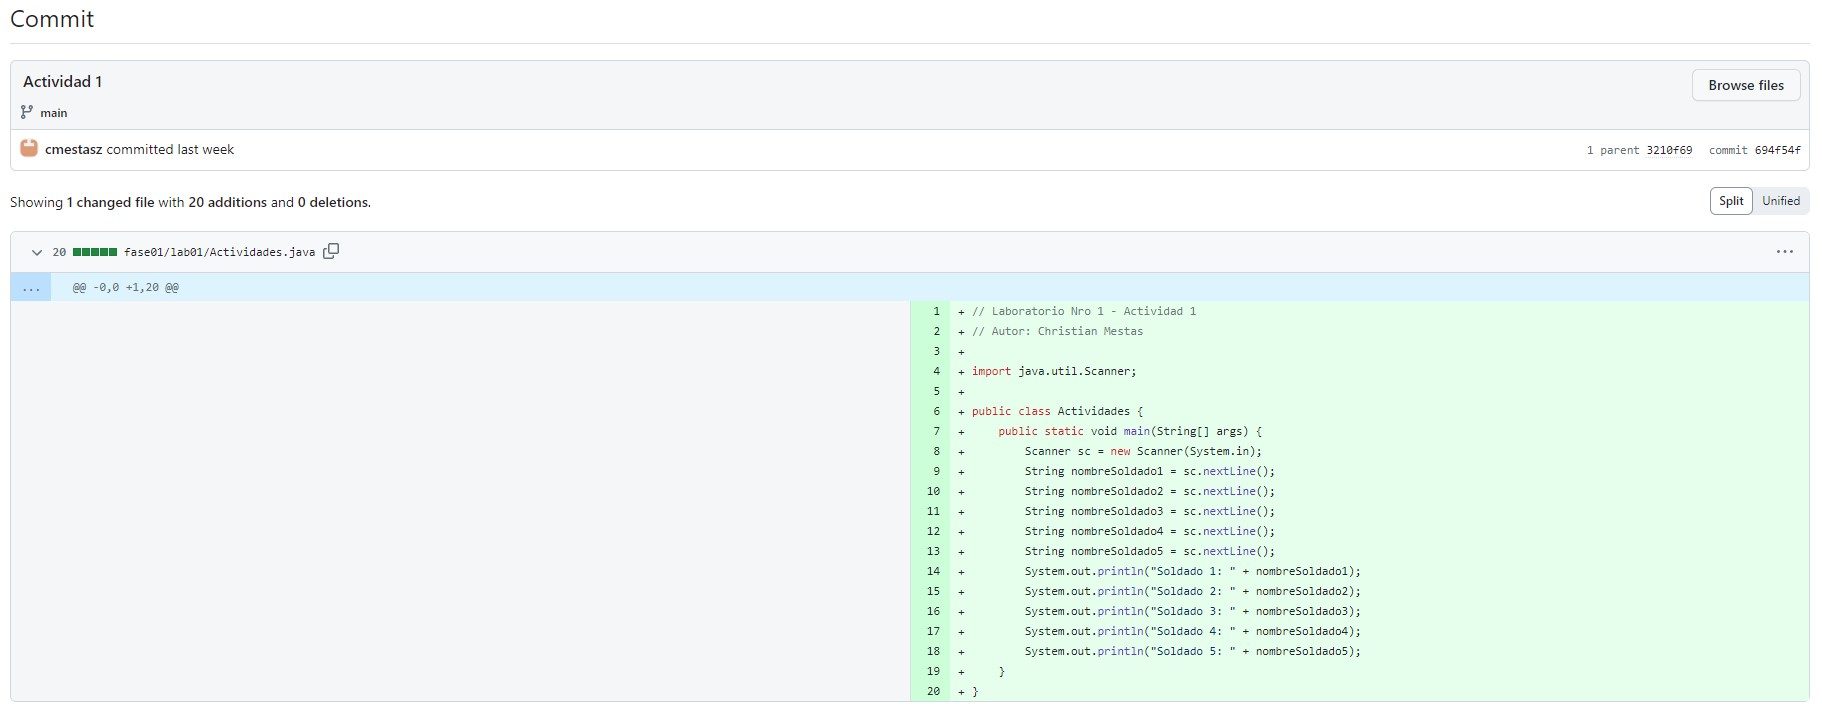
\includegraphics[width=1\textwidth,keepaspectratio]{img/commit03.jpg}
	\caption{Tercer Commit.}
\end{figure}
\begin{figure}[H]
	\centering
	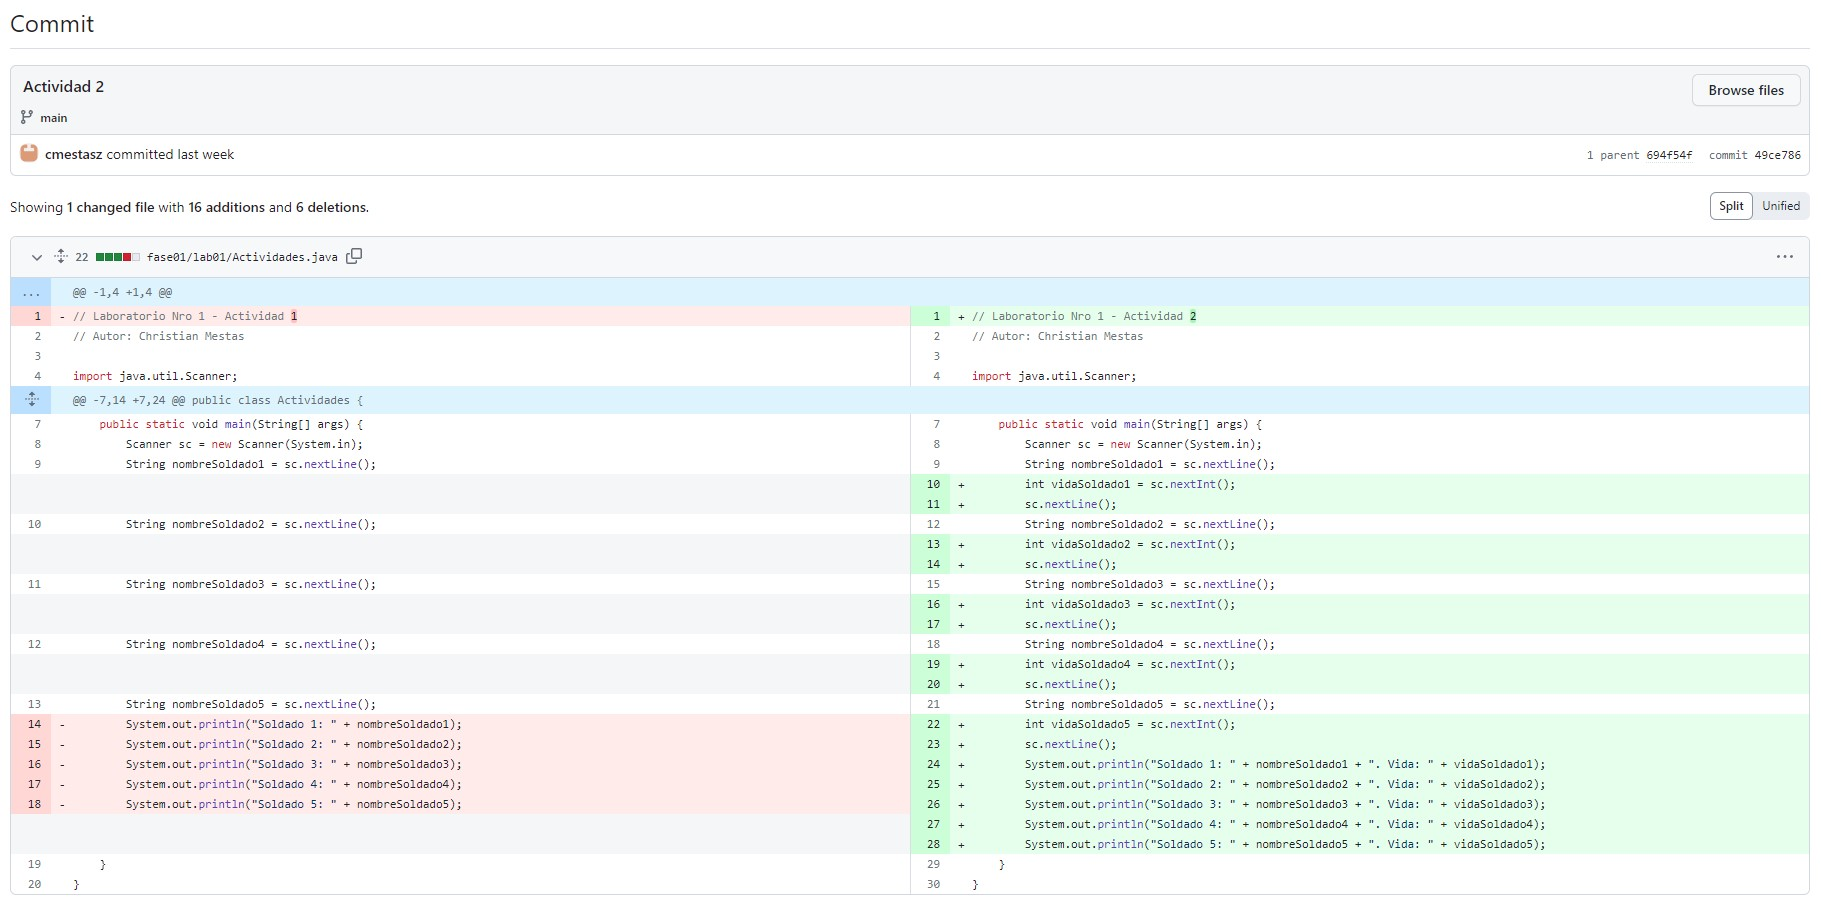
\includegraphics[width=1\textwidth,keepaspectratio]{img/commit04.jpg}
	\caption{Cuarto Commit.}
\end{figure}
\begin{figure}[H]
	\centering
	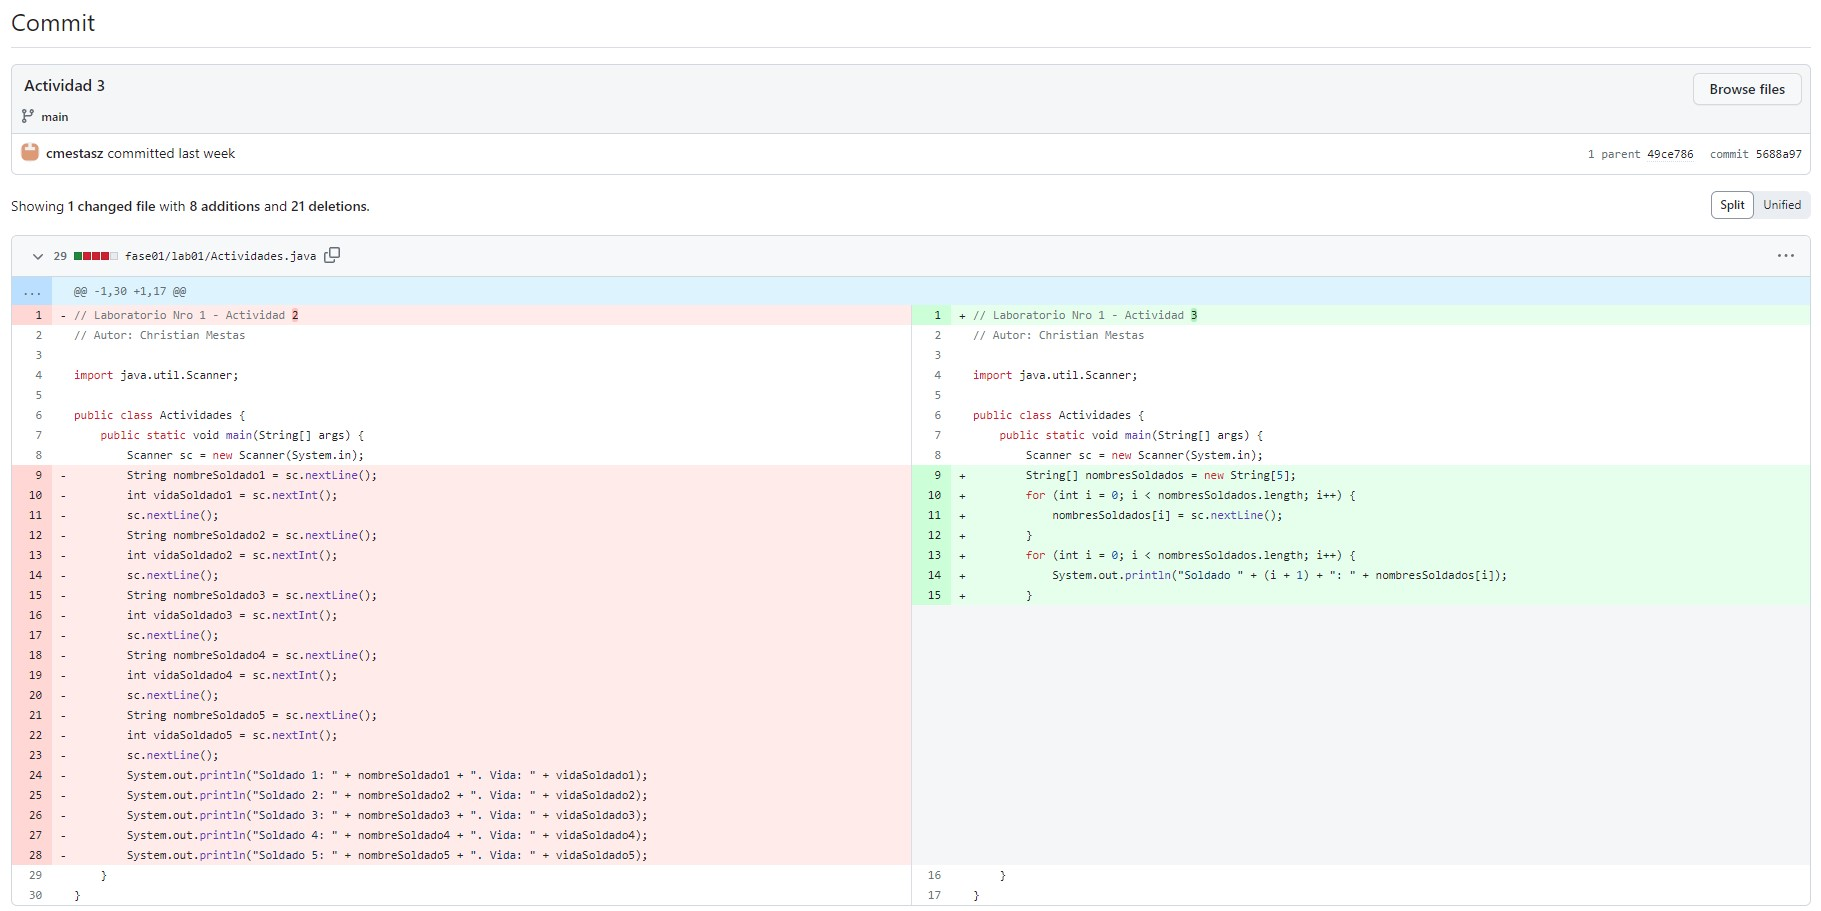
\includegraphics[width=1\textwidth,keepaspectratio]{img/commit05.jpg}
	\caption{Quinto Commit.}
\end{figure}
\begin{figure}[H]
	\centering
	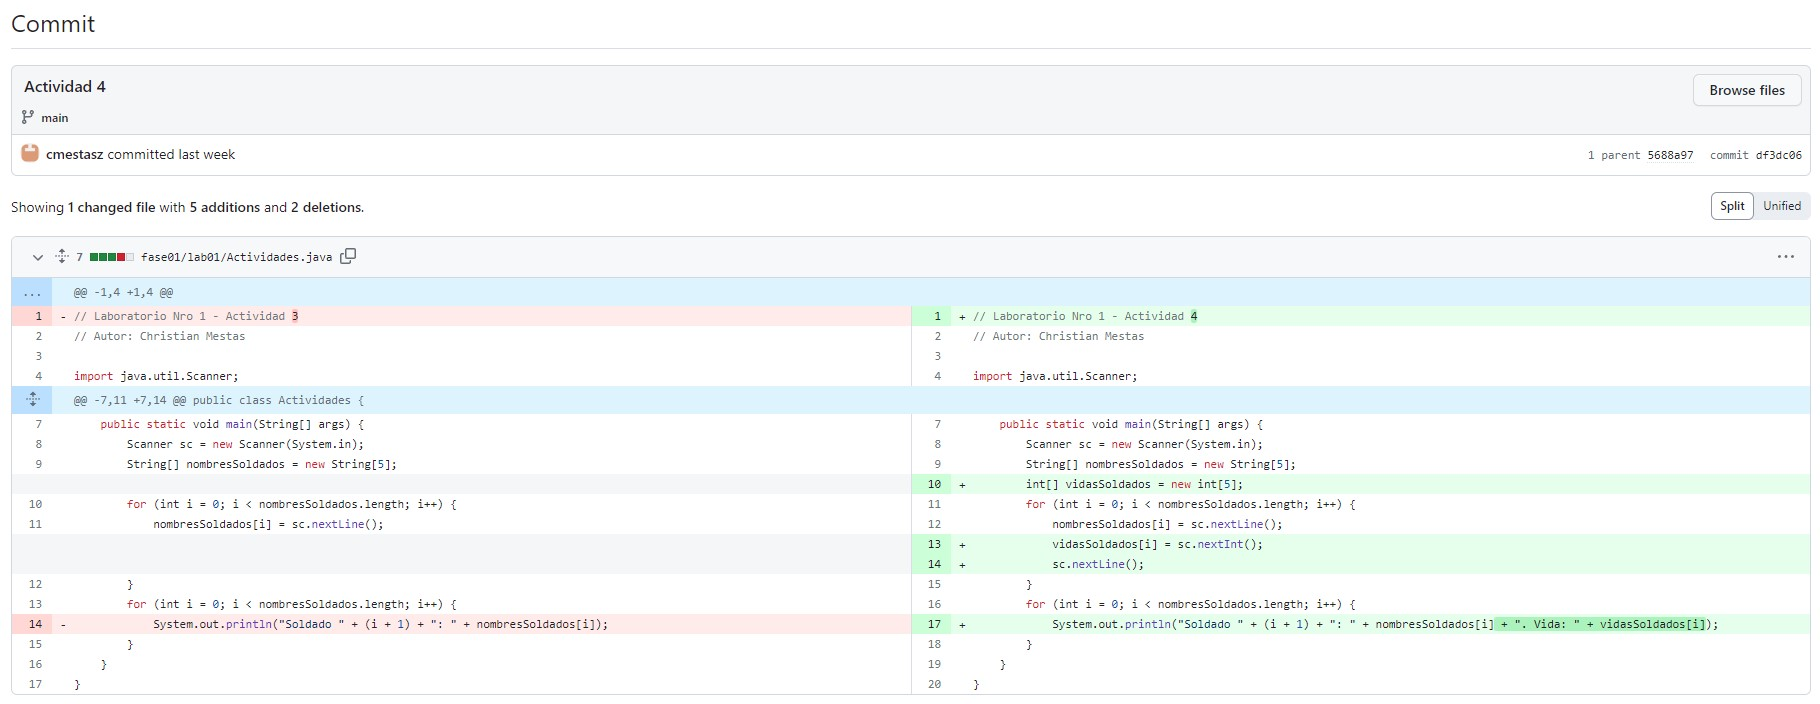
\includegraphics[width=1\textwidth,keepaspectratio]{img/commit06.jpg}
	\caption{Sexto Commit.}
\end{figure}
\begin{figure}[H]
	\centering
	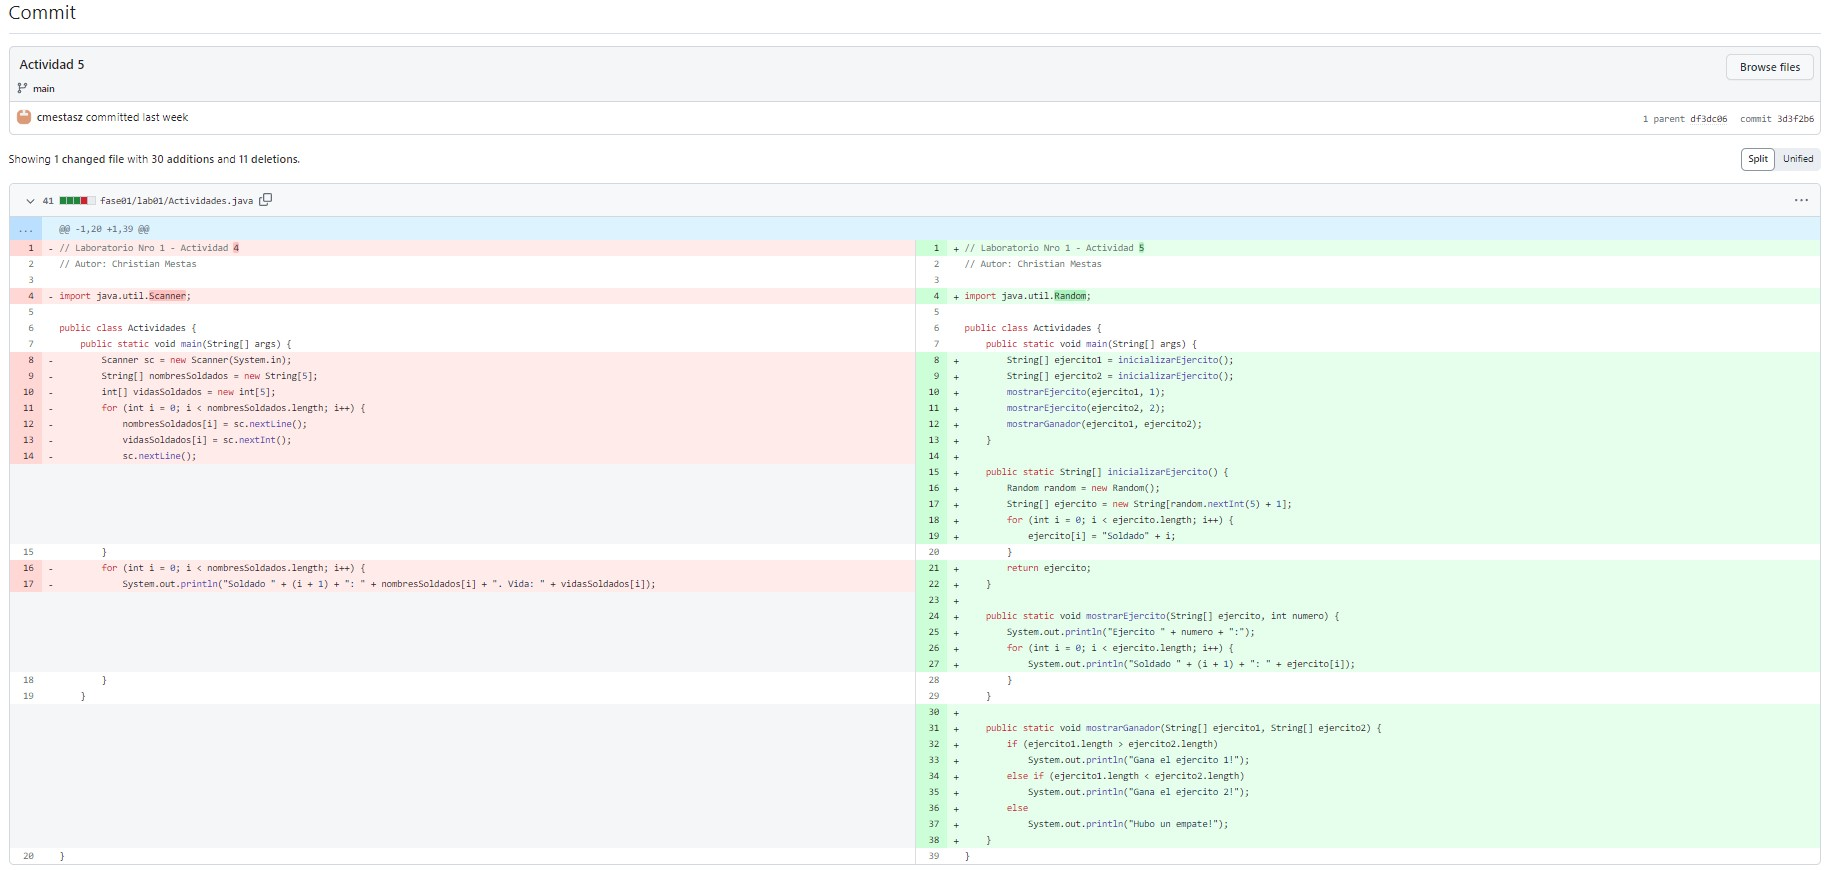
\includegraphics[width=1\textwidth,keepaspectratio]{img/commit07.jpg}
	\caption{Séptimo Commit.}
\end{figure}
\begin{lstlisting}[language=bash,caption={Actualizando .gitignore}]
		$ cd ../..
		$ code .gitignore
	\end{lstlisting}
\begin{lstlisting}[language=bash,caption={Octavo Commit / .gitignore}]
		$ git add .gitignore
		$ git commit -m "Actualizar .gitignore para que ignore los archivos generados por la compilacion latex"
		$ git push
	\end{lstlisting}
\begin{figure}[H]
	\centering
	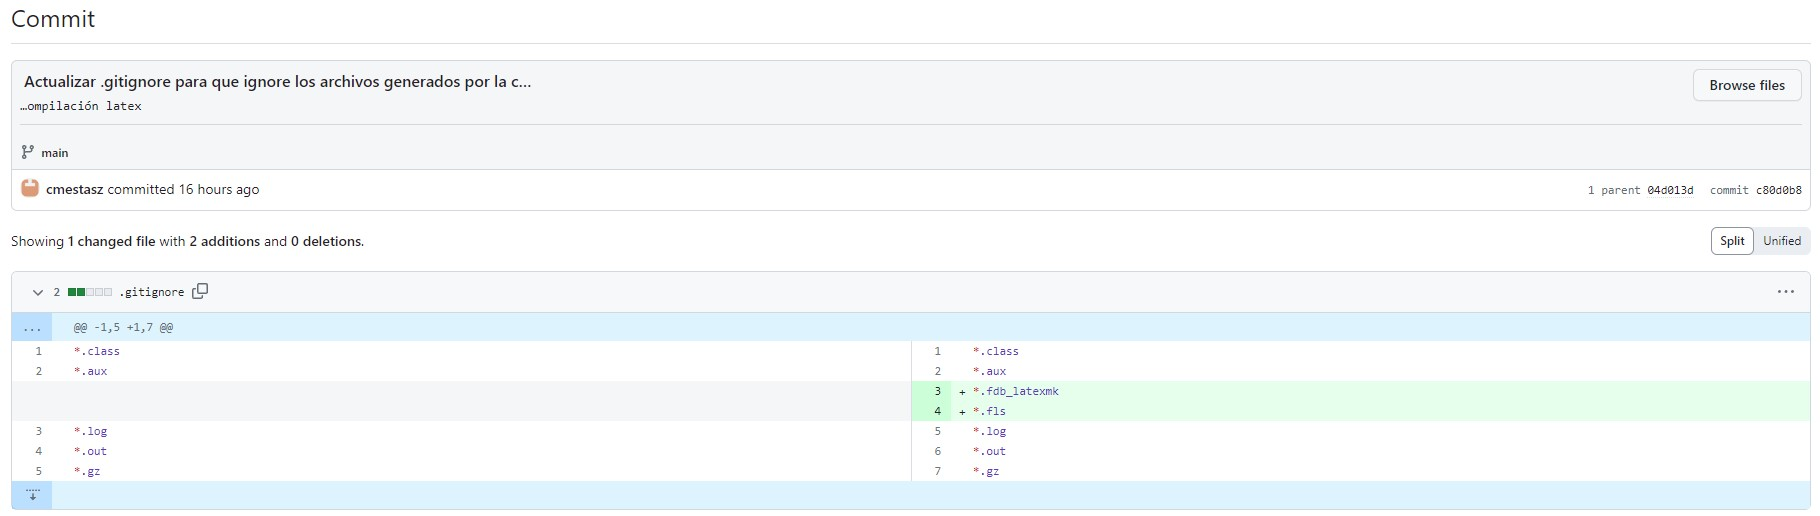
\includegraphics[width=1\textwidth,keepaspectratio]{img/commit08.jpg}
	\caption{Octavo Commit.}
\end{figure}

\pagebreak
\section{Código desarrollado}
\lstinputlisting[language=bash, caption={.gitignore},numbers=left,]{src/.gitignore}
\lstinputlisting[language=Java, caption={Actividades.java (Actividad 1)},numbers=left,]{src/Actividad1.java}
\begin{itemize}
	\item Los 5 nombres son leídos linea por linea y guardados en 5 variables diferentes.
	\item Luego los datos son impresos linea por linea en el mismo orden en el que se ingresaron.
\end{itemize}
\pagebreak
\lstinputlisting[language=Java, caption={Actividades.java (Actividad 2)},numbers=left,]{src/Actividad2.java}
\begin{itemize}
	\item Los 5 nombres y sus respectivas vidas son leídas linea por linea y guardadas en 5 variables diferentes por atributo.
	\item Luego los datos son impresos linea por linea en el mismo orden en el que se ingresaron.
\end{itemize}
\pagebreak
\lstinputlisting[language=Java, caption={Actividades.java (Actividad 3)},numbers=left,]{src/Actividad3.java}
\begin{itemize}
	\item Los 5 nombres son leídos iterativamente y guardados en un arreglo.
	\item Luego los datos son impresos iterativamente en el mismo orden en el que se ingresaron.
\end{itemize}
\lstinputlisting[language=Java, caption={Actividades.java (Actividad 4)},numbers=left,]{src/Actividad4.java}
\begin{itemize}
	\item Los 5 nombres y sus respectivas vidas son leídas iterativamente y guardadas en 2 arreglos.
	\item Luego los datos son impresos iterativamente en el mismo orden en el que se ingresaron.
\end{itemize}
\pagebreak
\lstinputlisting[language=Java, caption={Actividades.java (Actividad 5)},numbers=left,]{src/Actividad5.java}
\begin{itemize}
	\item Se crean 2 ejércitos con el método inicializarEjercito(), que crea un ejército de tamaño al azar entre 1 y 5.
	\item Se muestran los ejércitos con el método mostrarEjercito(), que imprime una lista de los soldados del ejército.
	\item Se muestra el ganador con el método mostrarGanador(), que compara los tamaños de los ejércitos y declara al ganador como el ejército mas grande.
\end{itemize}
\pagebreak

\section{Ejecución del código}
\begin{figure}[H]
	\centering
	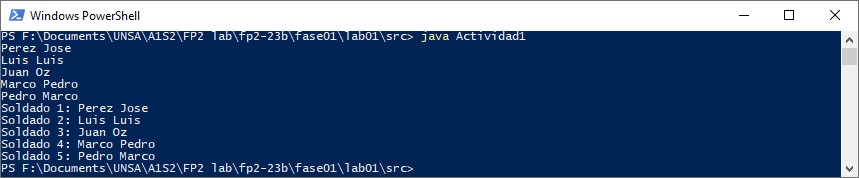
\includegraphics[width=1\textwidth,keepaspectratio]{img/ejec01.jpg}
	\caption{Actividad 1}
\end{figure}
\begin{figure}[H]
	\centering
	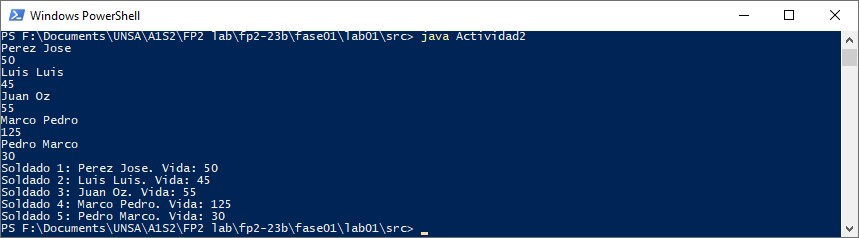
\includegraphics[width=1\textwidth,keepaspectratio]{img/ejec02.jpg}
	\caption{Actividad 2}
\end{figure}
\begin{figure}[H]
	\centering
	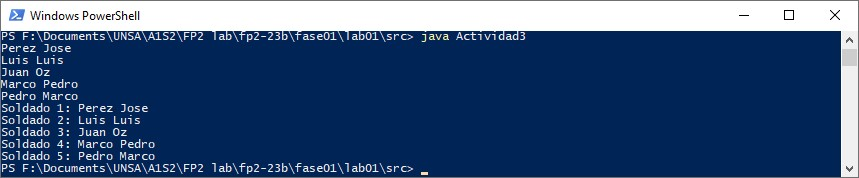
\includegraphics[width=1\textwidth,keepaspectratio]{img/ejec03.jpg}
	\caption{Actividad 3}
\end{figure}
\begin{figure}[H]
	\centering
	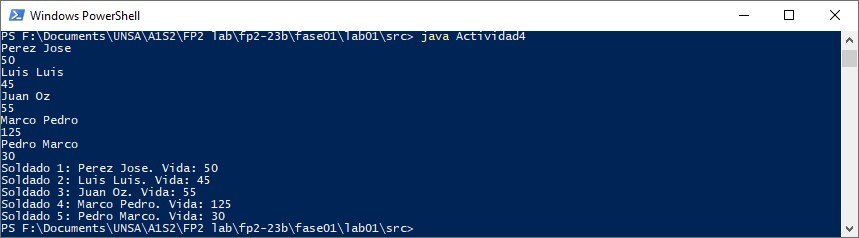
\includegraphics[width=1\textwidth,keepaspectratio]{img/ejec04.jpg}
	\caption{Actividad 4}
\end{figure}
\begin{figure}[H]
	\centering
	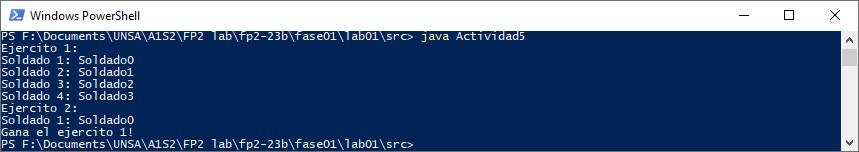
\includegraphics[width=1\textwidth,keepaspectratio]{img/ejec05.jpg}
	\caption{Actividad 5}
\end{figure}
\clearpage

\section{Estructura de laboratorio 01}
\begin{itemize}
	\item El contenido que se entrega en este laboratorio es el siguiente:
\end{itemize}

\begin{lstlisting}[style=ascii-tree]
lab01/
|--- VideoJuego.java
|--- Actividades.java
|--- Informe.tex
|--- Informe.pdf
|--- img
	|--- logo_abet.png
	|--- logo_episunsa.png
	|--- logo_unsa.jpg
	|--- commit01.jpg
	|--- commit02.jpg
	|--- commit03.jpg
	|--- commit04.jpg
	|--- commit05.jpg
	|--- commit06.jpg
	|--- commit07.jpg
	|--- commit08.jpg
	|--- ejec01.jpg
	|--- ejec02.jpg
	|--- ejec03.jpg
	|--- ejec04.jpg
	|--- ejec05.jpg
|--- src  
	|--- .gitignore
	|--- Actividad1.java
	|--- Actividad2.java
	|--- Actividad3.java
	|--- Actividad4.java
	|--- Actividad5.java
\end{lstlisting}
\pagebreak

\section{\textcolor{red}{Rúbricas}}

\subsection{\textcolor{red}{Entregable Informe}}
\begin{table}[H]
	\caption{Tipo de Informe}
	\setlength{\tabcolsep}{0.5em} % for the horizontal padding
	{\renewcommand{\arraystretch}{1.5}% for the vertical padding
		\begin{tabular}{|M{3cm}|M{12cm}|}
			\hline
			\multicolumn{2}{|c|}{\textbf{\textcolor{red}{Informe}}}                                                                                                      \\
			\hline
			\textbf{\textcolor{red}{Latex}} & \textcolor{blue}{El informe está en formato PDF desde Latex,  con un formato limpio (buena presentación) y facil de leer.} \\
			\hline
		\end{tabular}
	}
\end{table}

\subsection{\textcolor{red}{Rúbrica para el contenido del Informe y demostración}}
\begin{itemize}
	\item El alumno debe marcar o dejar en blanco en celdas de la columna \textbf{Checklist} si cumplio con el ítem correspondiente.
	\item Si un alumno supera la fecha de entrega, su calificación será sobre la nota mínima aprobatoria, siempre y cuando cumpla con todos los items.
	\item El alumno debe autocalificarse en la columna \textbf{Estudiante} de acuerdo a la siguiente tabla:

	      \begin{table}[ht]
		      \caption{Niveles de desempeño}
		      \begin{center}
			      \begin{tabular}{ccccc}
				      \hline
				                      & \multicolumn{4}{c}{Nivel}                                                              \\
				      \cline{1-5}
				      \textbf{Puntos} & Insatisfactorio 25\%      & En Proceso 50\% & Satisfactorio 75\% & Sobresaliente 100\% \\
				      \textbf{2.0}    & 0.5                       & 1.0             & 1.5                & 2.0                 \\
				      \textbf{4.0}    & 1.0                       & 2.0             & 3.0                & 4.0                 \\
				      \hline
			      \end{tabular}
		      \end{center}
	      \end{table}

\end{itemize}

\begin{table}[H]
	\caption{Rúbrica para contenido del Informe y demostración}
	\setlength{\tabcolsep}{0.5em} % for the horizontal padding
	{\renewcommand{\arraystretch}{1.5}% for the vertical padding
		%\begin{center}
		\begin{tabular}{|M{2.3cm}|M{5cm}|M{1.2cm}|M{1.5cm}|M{1.8cm}|M{1.4cm}|}
			\hline
			\multicolumn{2}{|c|}{Contenido y demostración} 																																																					 & Puntos	 & Checklist  & Estudiante & Profesor   \\
			\hline
			\textbf{1. GitHub}                             & Hay enlace URL activo del directorio para el  laboratorio hacia su repositorio GitHub con código fuente terminado y fácil de revisar.                                                                           & 2         & X          & 2          & \\
			\hline
			\textbf{2. Commits}                            & Hay capturas de pantalla de los commits más importantes con sus explicaciones detalladas. (El profesor puede preguntar para refrendar calificación).                                                            & 4         & X          & 4          & \\
			\hline
			\textbf{3. Código fuente}                      & Hay porciones de código fuente importantes con numeración y explicaciones detalladas de sus funciones.                                                                                                          & 2         & X          & 2          & \\
			\hline
			\textbf{4. Ejecución}                          & Se incluyen ejecuciones/pruebas del código fuente  explicadas gradualmente.                                                                                                                                     & 2         & X          & 1.5        & \\
			\hline
			\textbf{5. Pregunta}                           & Se responde con completitud a la pregunta formulada en la tarea.  (El profesor puede preguntar para refrendar calificación).                                                                                    & 2         &            & 0          & \\
			\hline
			\textbf{6. Fechas}                             & Las fechas de modificación del código fuente estan dentro de los plazos de fecha de entrega establecidos.                                                                                                       & 2         & X          & 2          & \\
			\hline
			\textbf{7. Ortografía}                         & El documento no muestra errores ortográficos.                                                                                                                                                                   & 2         & X          & 2          & \\
			\hline
			\textbf{8. Madurez}                            & El Informe muestra de manera general una evolución de la madurez del código fuente,  explicaciones puntuales pero precisas y un acabado impecable.   (El profesor puede preguntar para refrendar calificación). & 4         & X          & 3          & \\
			\hline
			\multicolumn{2}{|c|}{\textbf{Total}}          																																																					 & 20		 &            & 16.5         &              \\
			\hline
		\end{tabular}
		%\end{center}
		%\label{tab:multicol}
	}
\end{table}

\section{Referencias}
\begin{itemize}
	\item Aedo, M. y Castro, E. (2021). FUNDAMENTOS DE PROGRAMACIÓN 2 - Tópicos de Programación Orientada a Objetos. Editorial UNSA.
\end{itemize}

%\pagebreak
%\bibliographystyle{apalike}
%\bibliographystyle{IEEEtranN}
%\bibliography{bibliography}

\end{document}